\section{Task2: System modelling}
\subsection{Activity Diagram}
\subsubsection{Print Document Module}
Hoạt động bắt đầu khi sinh viên đăng nhập và chọn giữa "Mua trang in" và "In tài liệu". Nếu sinh viên chọn "In tài liệu", hệ thống sẽ hiển thị giao diện để chọn tài liệu in. Sinh viên tải file lên, và nếu file không đúng định dạng, hệ thống sẽ hiển thị thông báo lỗi. Khi tài liệu được tải lên thành công, sinh viên chọn máy in từ danh sách có sẵn và thiết lập các thuộc tính in như kích thước giấy, số trang, chế độ in (một mặt/hai mặt), và số lượng bản in. Nếu không có máy in khả dụng, hệ thống sẽ thông báo "Máy in không có sẵn".
\\ \\
Sau đó, hệ thống kiểm tra số trang cần in so với số trang sinh viên hiện có. Nếu số trang in vượt quá số trang sinh viên có, hệ thống sẽ yêu cầu sinh viên mua thêm trang in hoặc giảm số lượng trang cần in. Để mua thêm trang in, hệ thống hiển thị giao diện thanh toán BKPay và khi thanh toán thành công, sinh viên quay lại bước thiết lập in. Nếu thanh toán thất bại, hệ thống sẽ hiển thị thông báo lỗi.
\\ \\
Khi mọi thông tin được xác nhận và số trang in đủ, hệ thống tiến hành lệnh in. Nếu in thành công, hệ thống hiển thị thông báo “In thành công”. Nếu gặp sự cố trong quá trình in, như hết giấy hoặc kẹt giấy, hệ thống sẽ hiển thị thông báo lỗi và yêu cầu sinh viên chọn máy in khác hoặc liên hệ hỗ trợ kỹ thuật. Hoạt động kết thúc khi quá trình in tài liệu hoàn tất.

\begin{figure}[htbp]
    \centering
    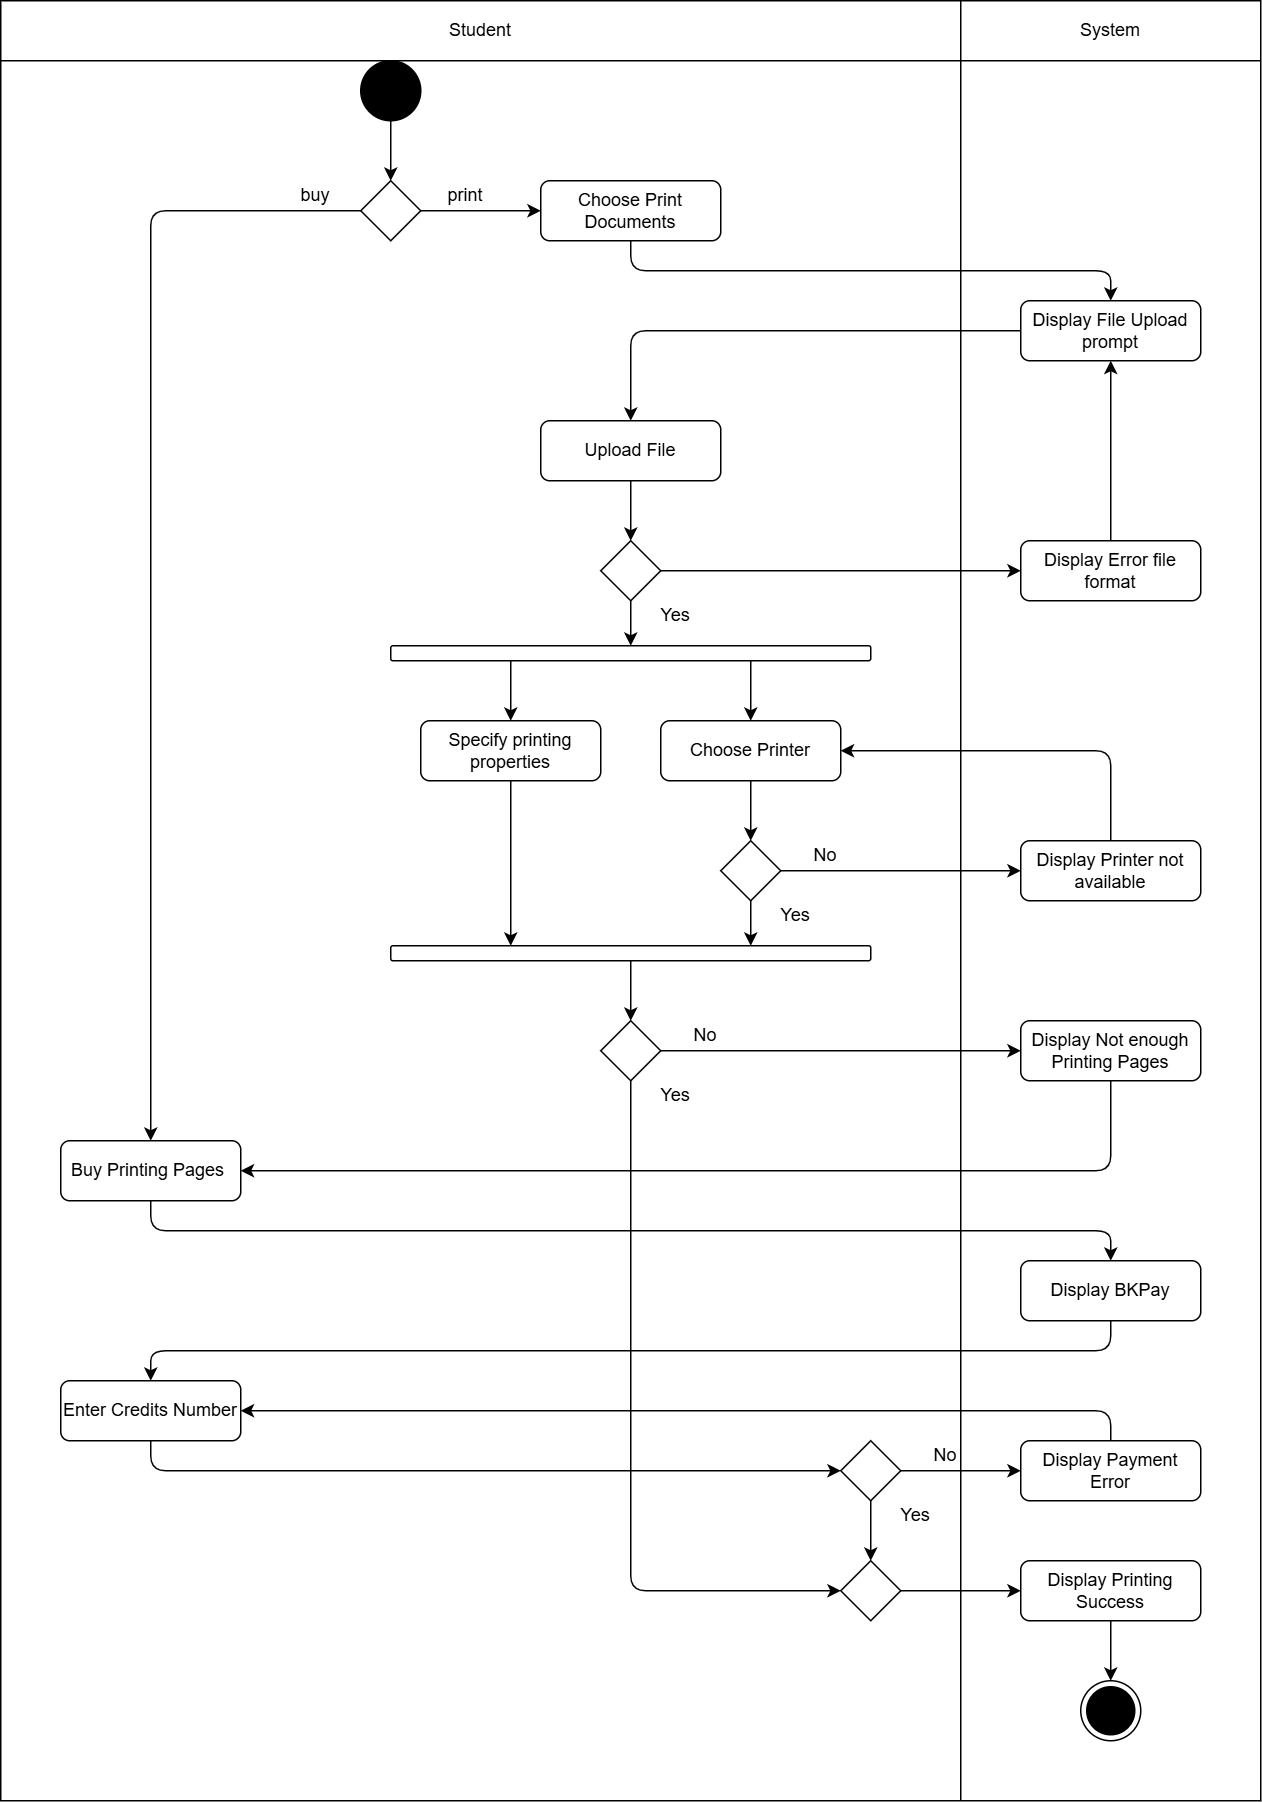
\includegraphics[width=0.9\textwidth]{Images/Activity/Print_activity.png}
    \caption{Activity Diagram for Print Document Module}
\end{figure}

\newpage
\subsubsection{Login Module}
Hoạt động bắt đầu khi User mở trang web và chọn "Đăng nhập". Hệ thống yêu cầu User phải chọn vai trò của mình, là Sinh viên hoặc SPSO. Sau khi User chọn vai trò, hệ thống yêu cầu User nhập thông tin đăng nhập, bao gồm tên đăng nhập và mật khẩu. Nếu thông tin không chính xác, hệ thống sẽ hiển thị thông báo lỗi và yêu cầu User nhập lại. Nếu thông tin chính xác, hệ thống sẽ chuyển User đến trang chính tương ứng với vai trò của User.

\begin{figure}[htbp]
    \centering
    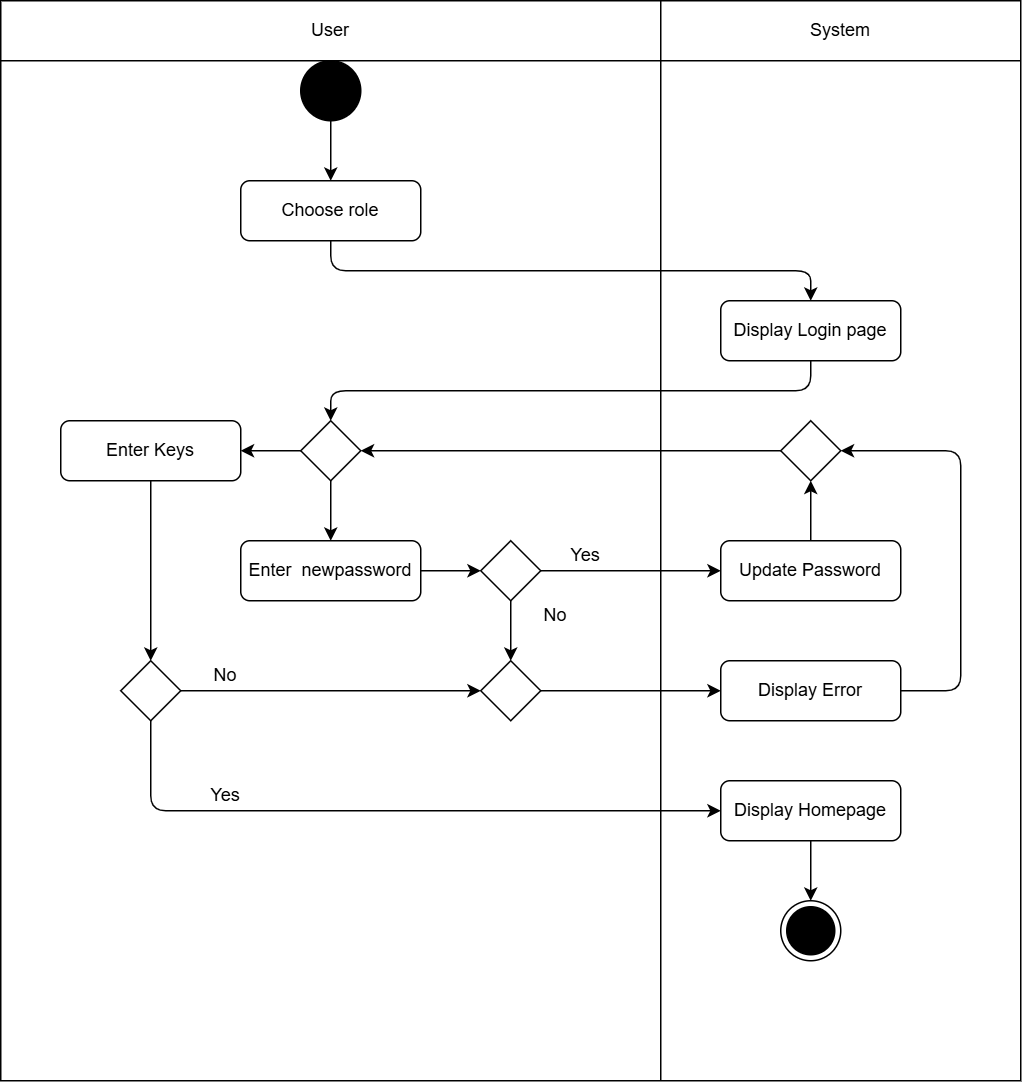
\includegraphics[width=0.9\textwidth]{Images/Activity/Login_activity.png}
    \caption{Activity Diagram for Login Module}
\end{figure}

\newpage
\subsubsection{Printer Management Module}
Hoạt động bắt đầu khi SPSO đăng nhập và có quyền quản lý máy in. SPSO chọn một máy in từ danh sách các máy đã kết nối và nhận diện bởi hệ thống. Hệ thống sẽ hiển thị chi tiết của máy in được chọn.
\\ \\
Tiếp theo, SPSO có thể lựa chọn kích hoạt hoặc vô hiệu hóa máy in. Hệ thống cập nhật trạng thái của máy in và hiển thị thông báo "Kích hoạt/Vô hiệu hóa thành công". Nếu không có máy in nào hiển thị trong danh sách hoặc SPSO muốn thêm máy in mới, SPSO chọn tùy chọn “Thêm máy in”. Hệ thống yêu cầu SPSO nhập thông tin máy in mới, bao gồm các thông số kỹ thuật cần thiết.
\\ \\
Sau khi SPSO nhập xong thông tin máy in, hệ thống cập nhật danh sách máy in với thông tin máy in mới và hiển thị thông báo "Thêm máy in thành công". Quá trình quản lý máy in hoàn tất khi SPSO hoàn thành các thao tác mong muốn.
\begin{figure}[htbp]
    \centering
    \includegraphics[width=0.9\textwidth]{Images/Activity/Printer_management_activity.png}
    \caption{Activity Diagram for Printer Management Module}
\end{figure}

\newpage
\subsubsection{Printing History Module}
Hoạt động bắt đầu khi sinh viên hoặc SPSO truy cập vào module lịch sử in ấn. Nếu là sinh viên, thì có thể chọn tùy chọn xem hồ sơ in ấn cá nhân để kiểm tra lịch sử in ấn và số trang in còn lại. SPSO sẽ truy cập trang lịch sử in ấn, nơi hệ thống sẽ hiển thị danh sách các lịch sử in ấn gần đây của sinh viên.
\\ \\
SPSO có thể chọn một bộ lọc thời gian để lọc lịch sử in ấn theo khoảng thời gian cụ thể. Hệ thống sẽ hiển thị lịch sử in ấn đã được lọc theo khoảng thời gian được chọn. SPSO cũng có thể chọn xem lịch sử in ấn của một sinh viên cụ thể. Hệ thống sẽ hiển thị toàn bộ lịch sử in ấn của sinh viên đó.
\\ \\
Ngoài ra, SPSO có thể chọn xem báo cáo thống kê in ấn. Hệ thống sẽ hiển thị chi tiết báo cáo, bao gồm thông tin tổng quan về số lượng và chi tiết in ấn theo thời gian. Hoạt động kết thúc sau khi người dùng hoàn tất việc xem thông tin.
\begin{figure}[htbp]
    \centering
    \includegraphics[width=0.9\textwidth]{Images/Activity/Printing_history_activity.png}
    \caption{Activity Diagram for Printing History Module}
\end{figure}

\newpage
\subsection{Sequence Diagram}
\textbf{Luồng Upload tài liệu:}
\begin{itemize}
    \item Sinh viên tải file lên thông qua Client:
    \begin{itemize}
        \item Client gửi request \texttt{POST /fileUpload} đến Controller.
        \item Controller gọi đến Model để thực hiện \texttt{Documents.upload()}.
        \item Model thực hiện query \texttt{INSERT} vào bảng documents trong Database.
    \end{itemize}
    \item Nếu thành công:
    \begin{itemize}
        \item Database trả về true.
        \item Hệ thống trả về status 200.
        \item Client hiển thị thông báo "Upload Success".
    \end{itemize}
    \item Nếu file không đúng định dạng:
    \begin{itemize}
        \item Hệ thống trả về status 400.
        \item Client hiển thị "File Format Error".
    \end{itemize}
\end{itemize}

\textbf{Luồng Kiểm tra số trang in:}
\begin{itemize}
    \item Sinh viên chọn thuộc tính in (Select Printing Properties):
    \begin{itemize}
        \item Client gửi request \texttt{POST /print} đến Controller.
        \item Controller gọi \texttt{Student.getPrintingPage()} để kiểm tra số trang có thể in.
        \item Model query \texttt{SELECT pages} từ bảng student trong Database.
    \end{itemize}
    \item Nếu đủ số trang:
    \begin{itemize}
        \item Model thực hiện \texttt{Document.print()}.
        \item Database cập nhật bảng student và insert vào bảng logs.
        \item Hệ thống trả về status 200.
        \item Client hiển thị "Print Success".
    \end{itemize}
    \item Nếu không đủ số trang:
    \begin{itemize}
        \item Hệ thống trả về status 400.
        \item Client hiển thị "Not Enough Printing Page".
    \end{itemize}
\end{itemize}

\textbf{Luồng Mua thêm số trang:}
\begin{itemize}
    \item Sinh viên nhập số trang cần mua (Enter Number of Pages to Buy):
    \begin{itemize}
        \item Client gửi request \texttt{POST /buyPages} đến Controller.
        \item Controller gọi đến BKPay để thực hiện \texttt{await Payment()}.
    \end{itemize}
    \item Sau khi thanh toán hoàn tất (Complete Payment):
    \begin{itemize}
        \item BKPay trả về \texttt{Promise true}.
        \item Model thực hiện \texttt{Student.Buy()}.
        \item Database cập nhật \texttt{student.pages}.
        \item Hệ thống trả về status 200.
        \item Client hiển thị "Buy Success".
    \end{itemize}
\end{itemize}


\begin{figure}[htbp]
    \centering
    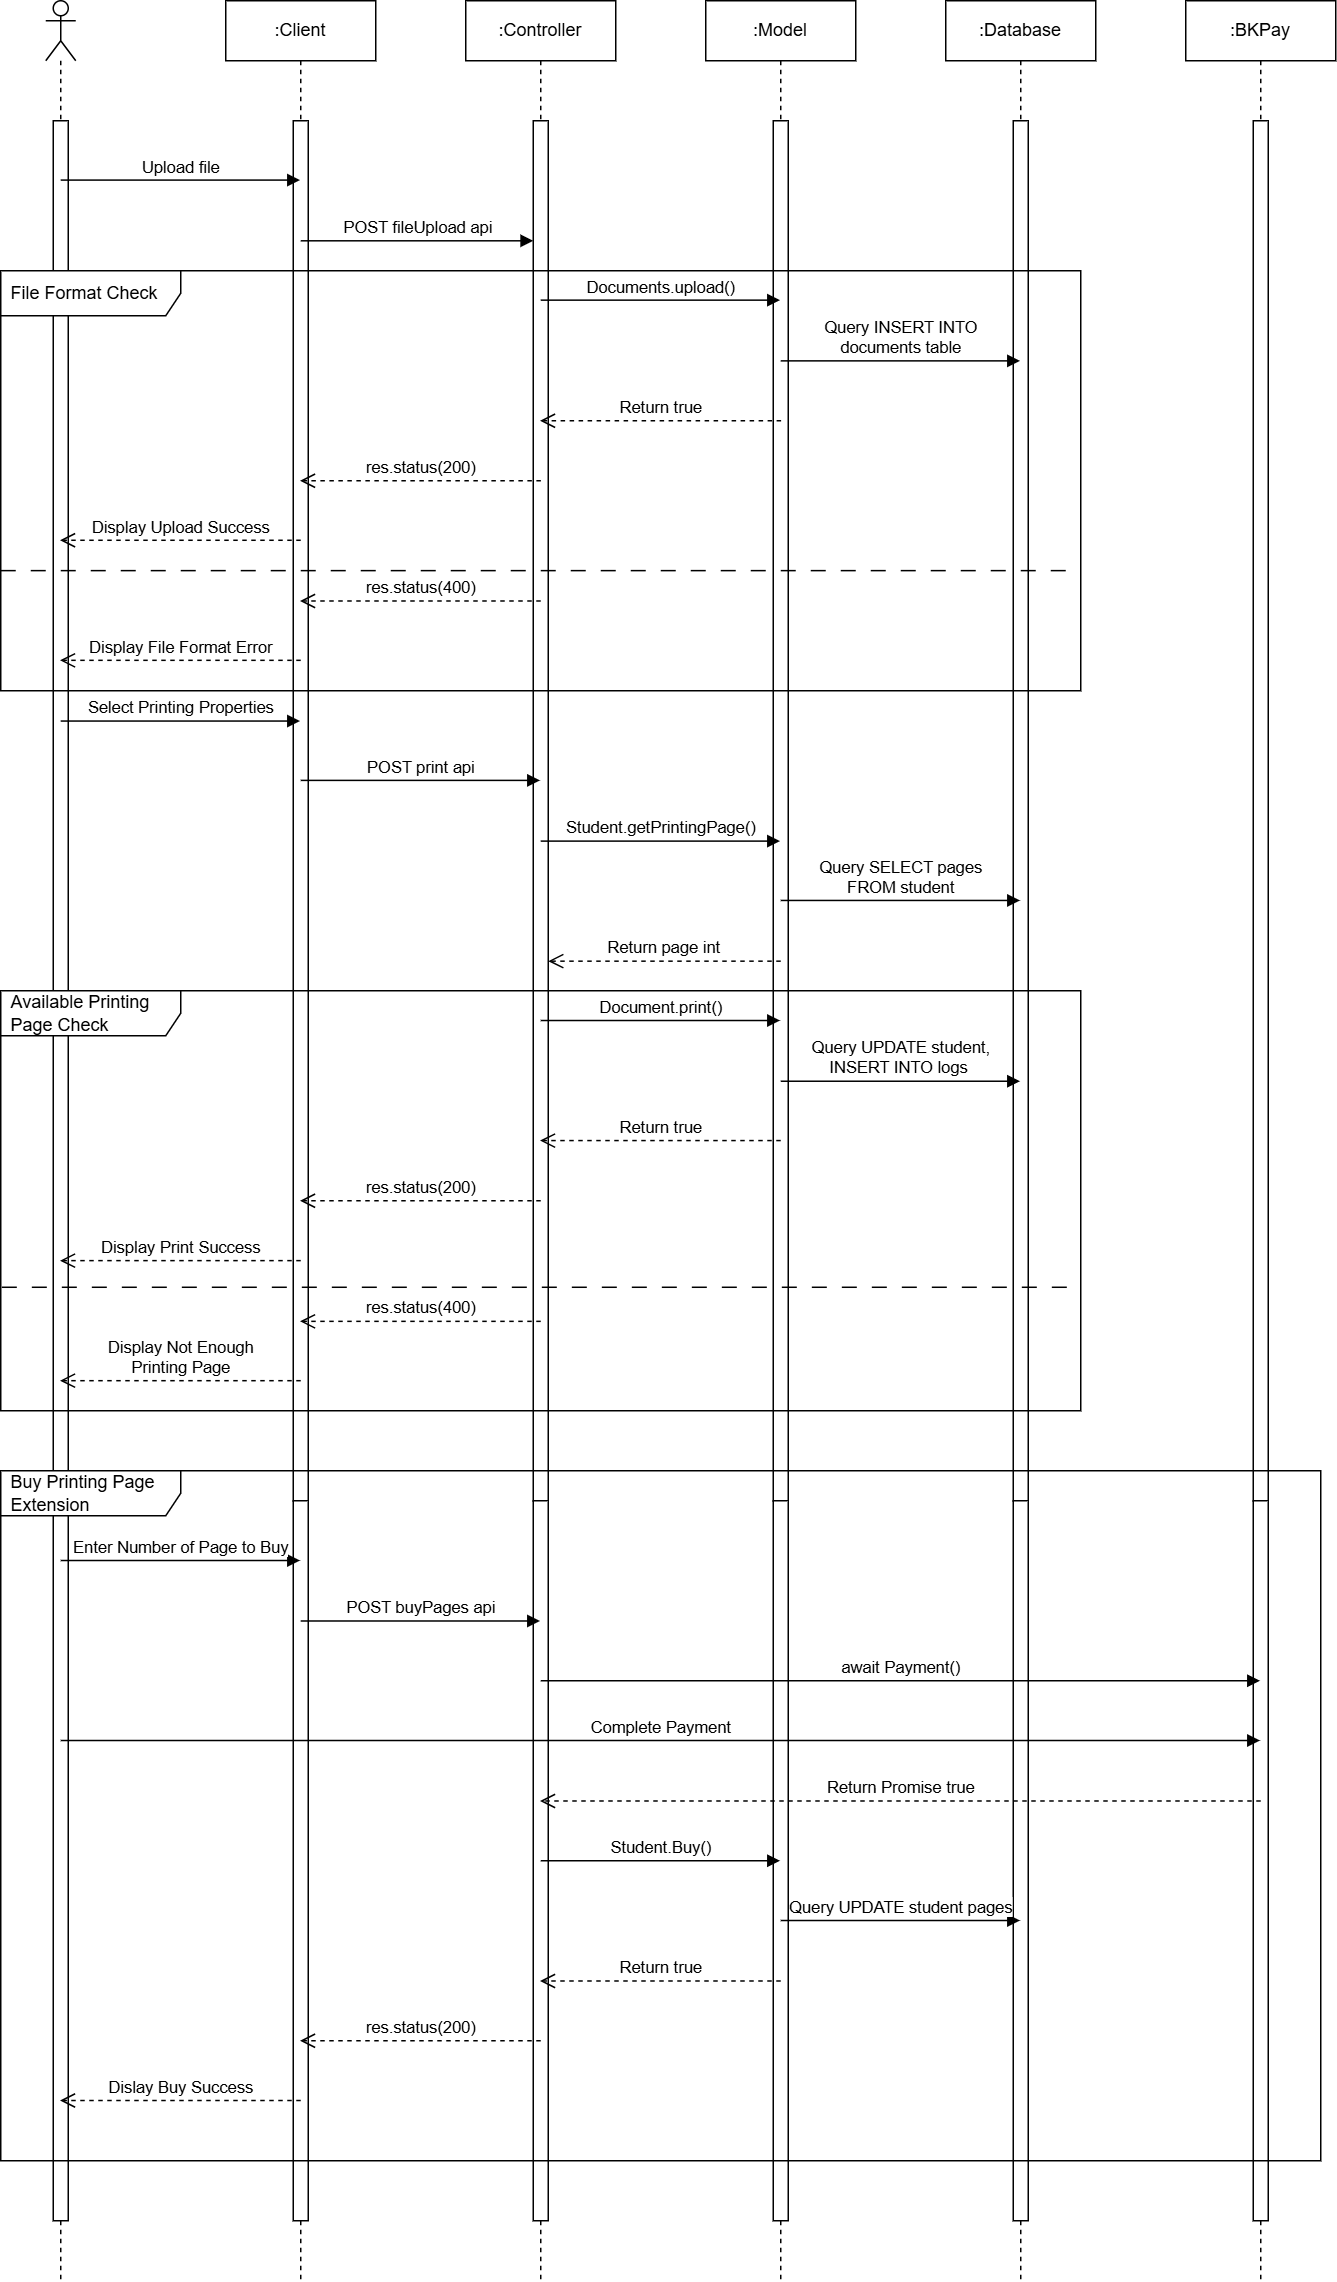
\includegraphics[width=0.8\textwidth]{Images/Diagrams/Print_sequence.png}
    \caption{Sequence Diagram for Print Document Module}
\end{figure}

\newpage
\subsection{Class Diagram}
% TODO add Class_diagram.png and comment out this section

 \begin{figure}[htbp]
     \centering
     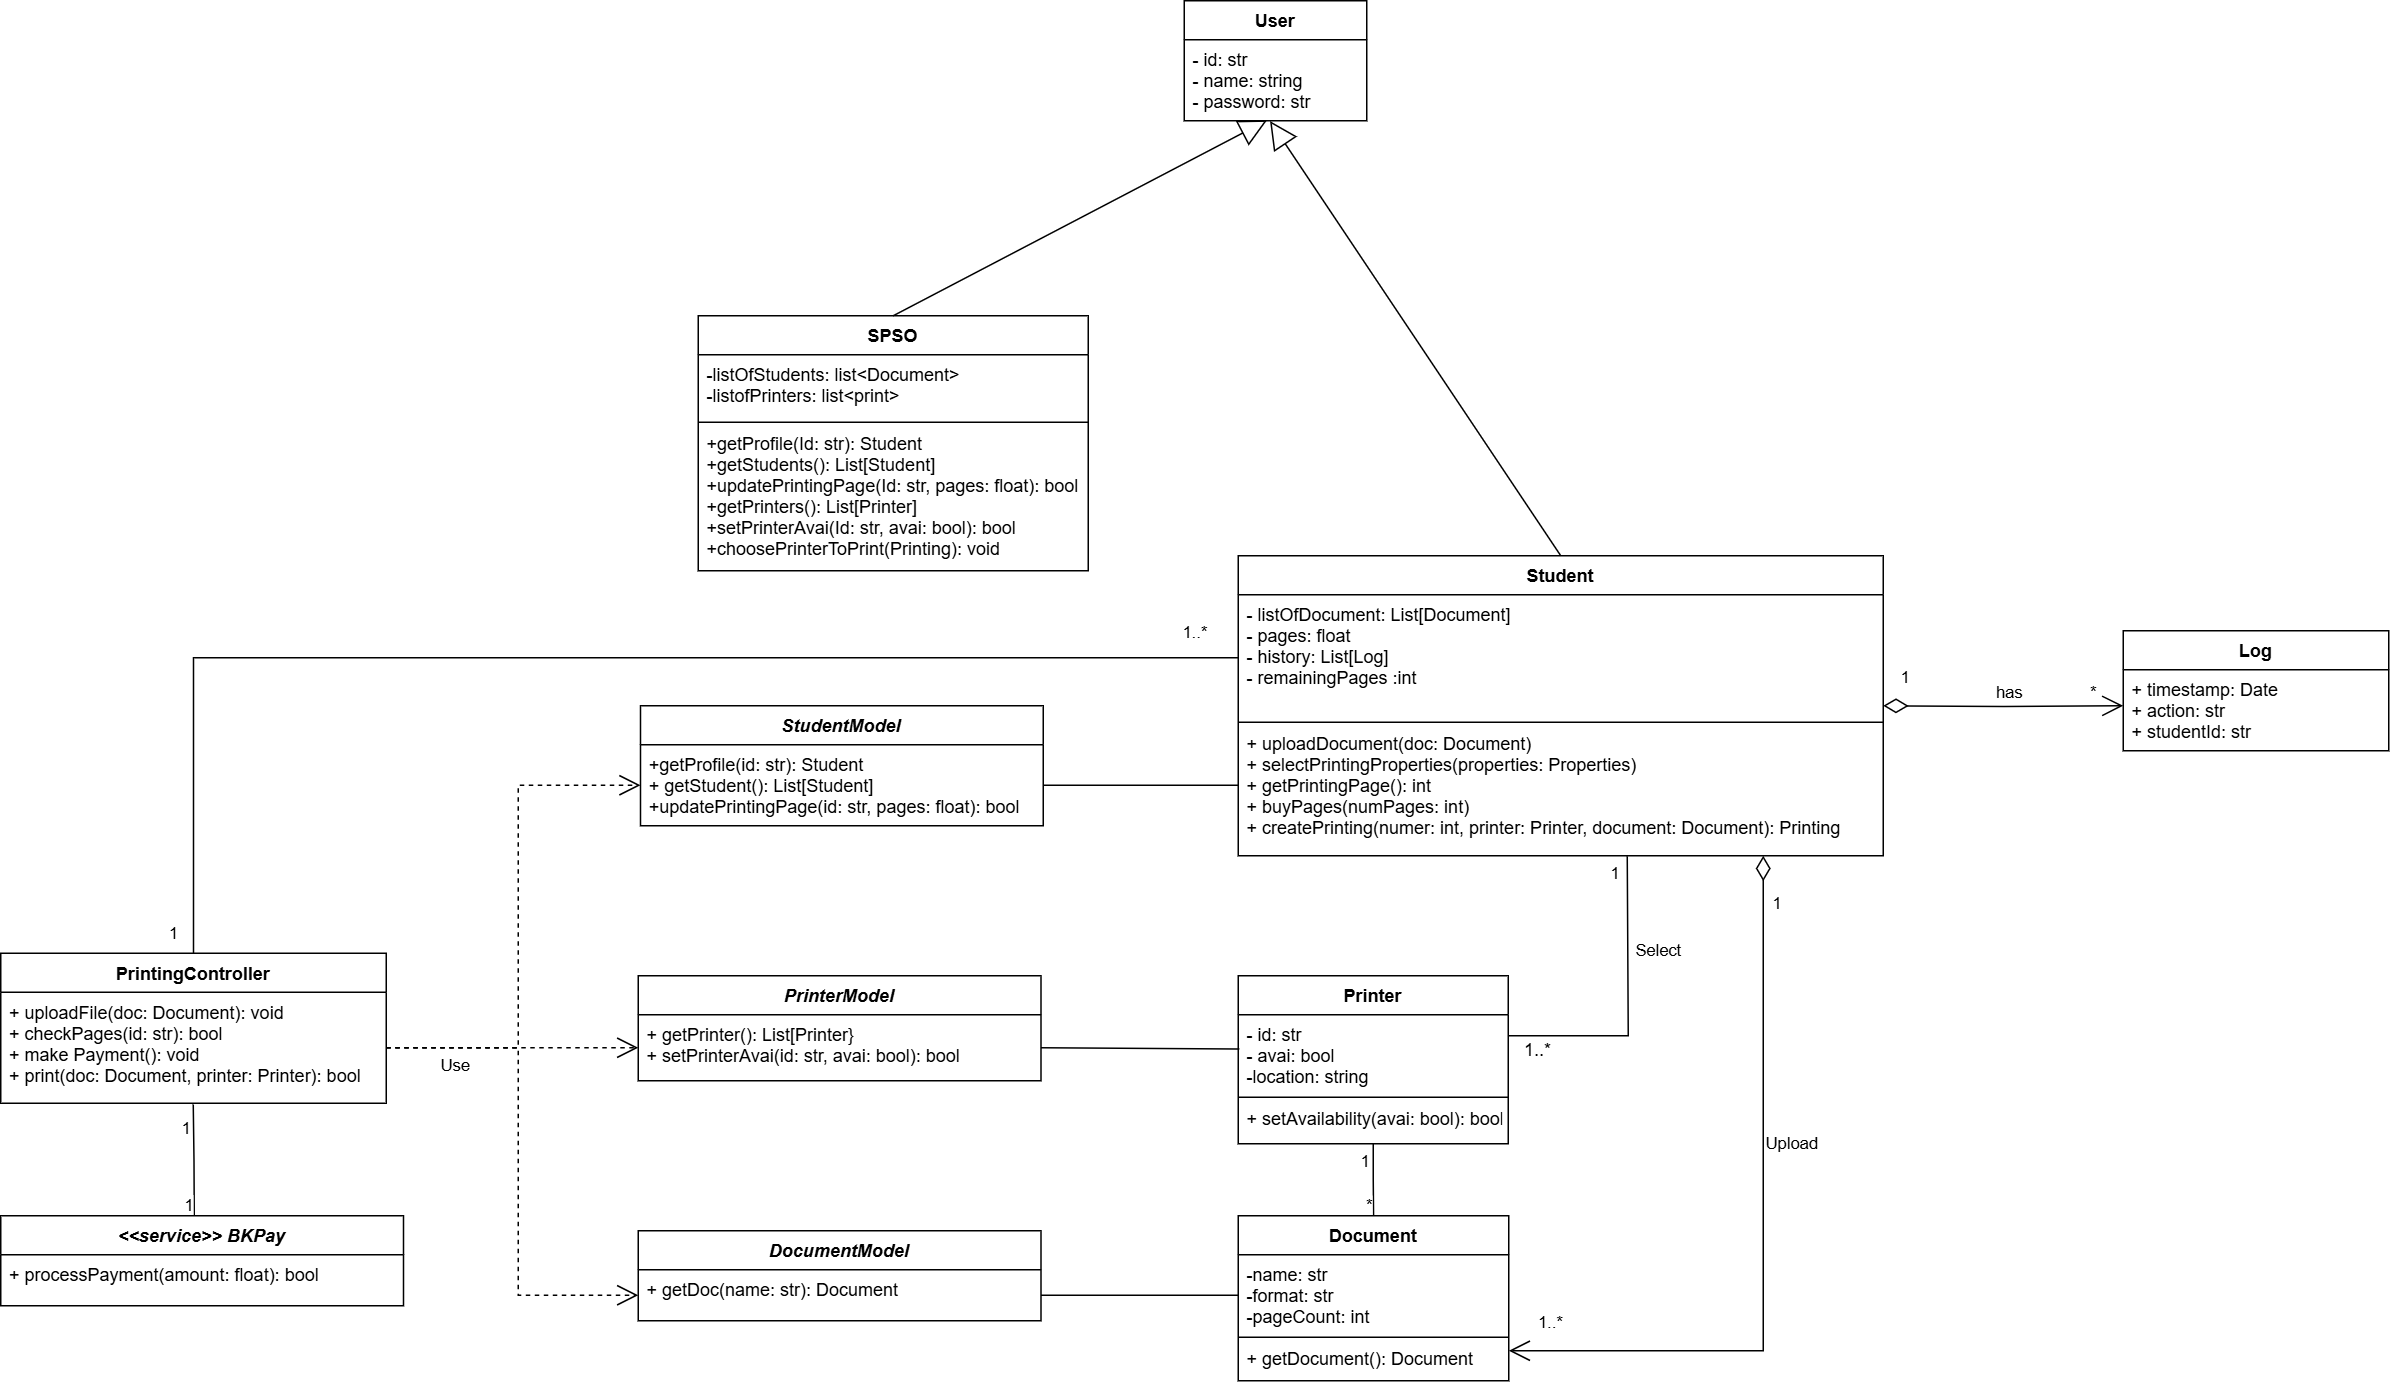
\includegraphics[width=1\linewidth]{Images/Diagrams/Class_diagram.png}
     \caption{Class Diagram}
 \end{figure}


\newpage
\section{UI Design}
\subsection{SPSO}
\subsubsection{Printer Management Page}
\begin{figure}[htbp]
     \centering
     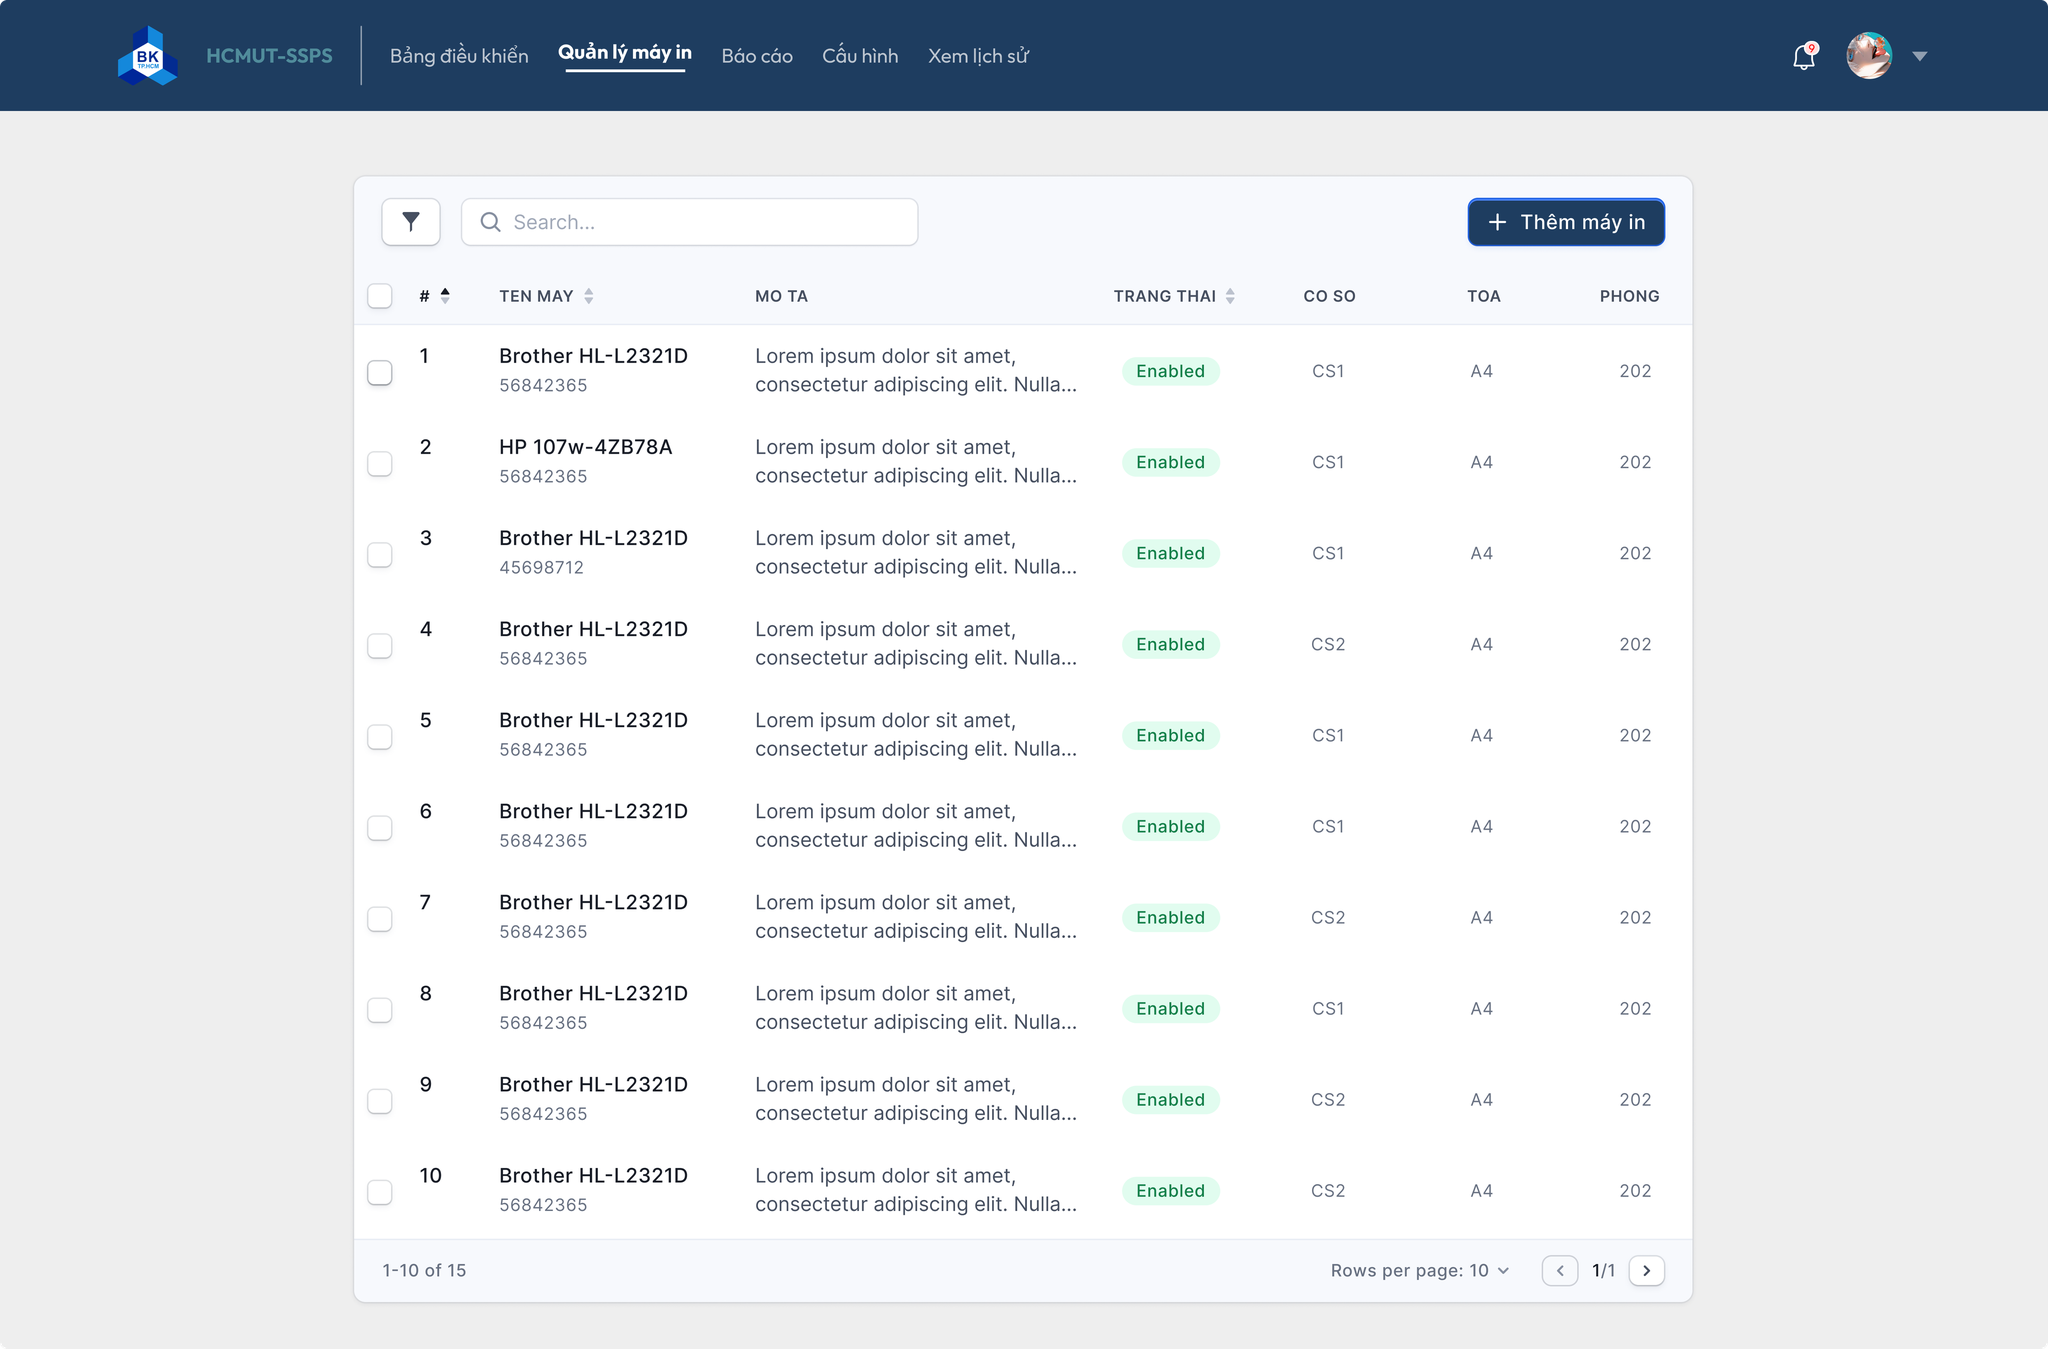
\includegraphics[width=1\linewidth]{Images/UI/Printer_Management.png}
     \caption{Printer Management Page}
 \end{figure} 
\newpage
\subsubsection{View Students' Printing History Page}

\begin{figure}[htbp]
     \centering
     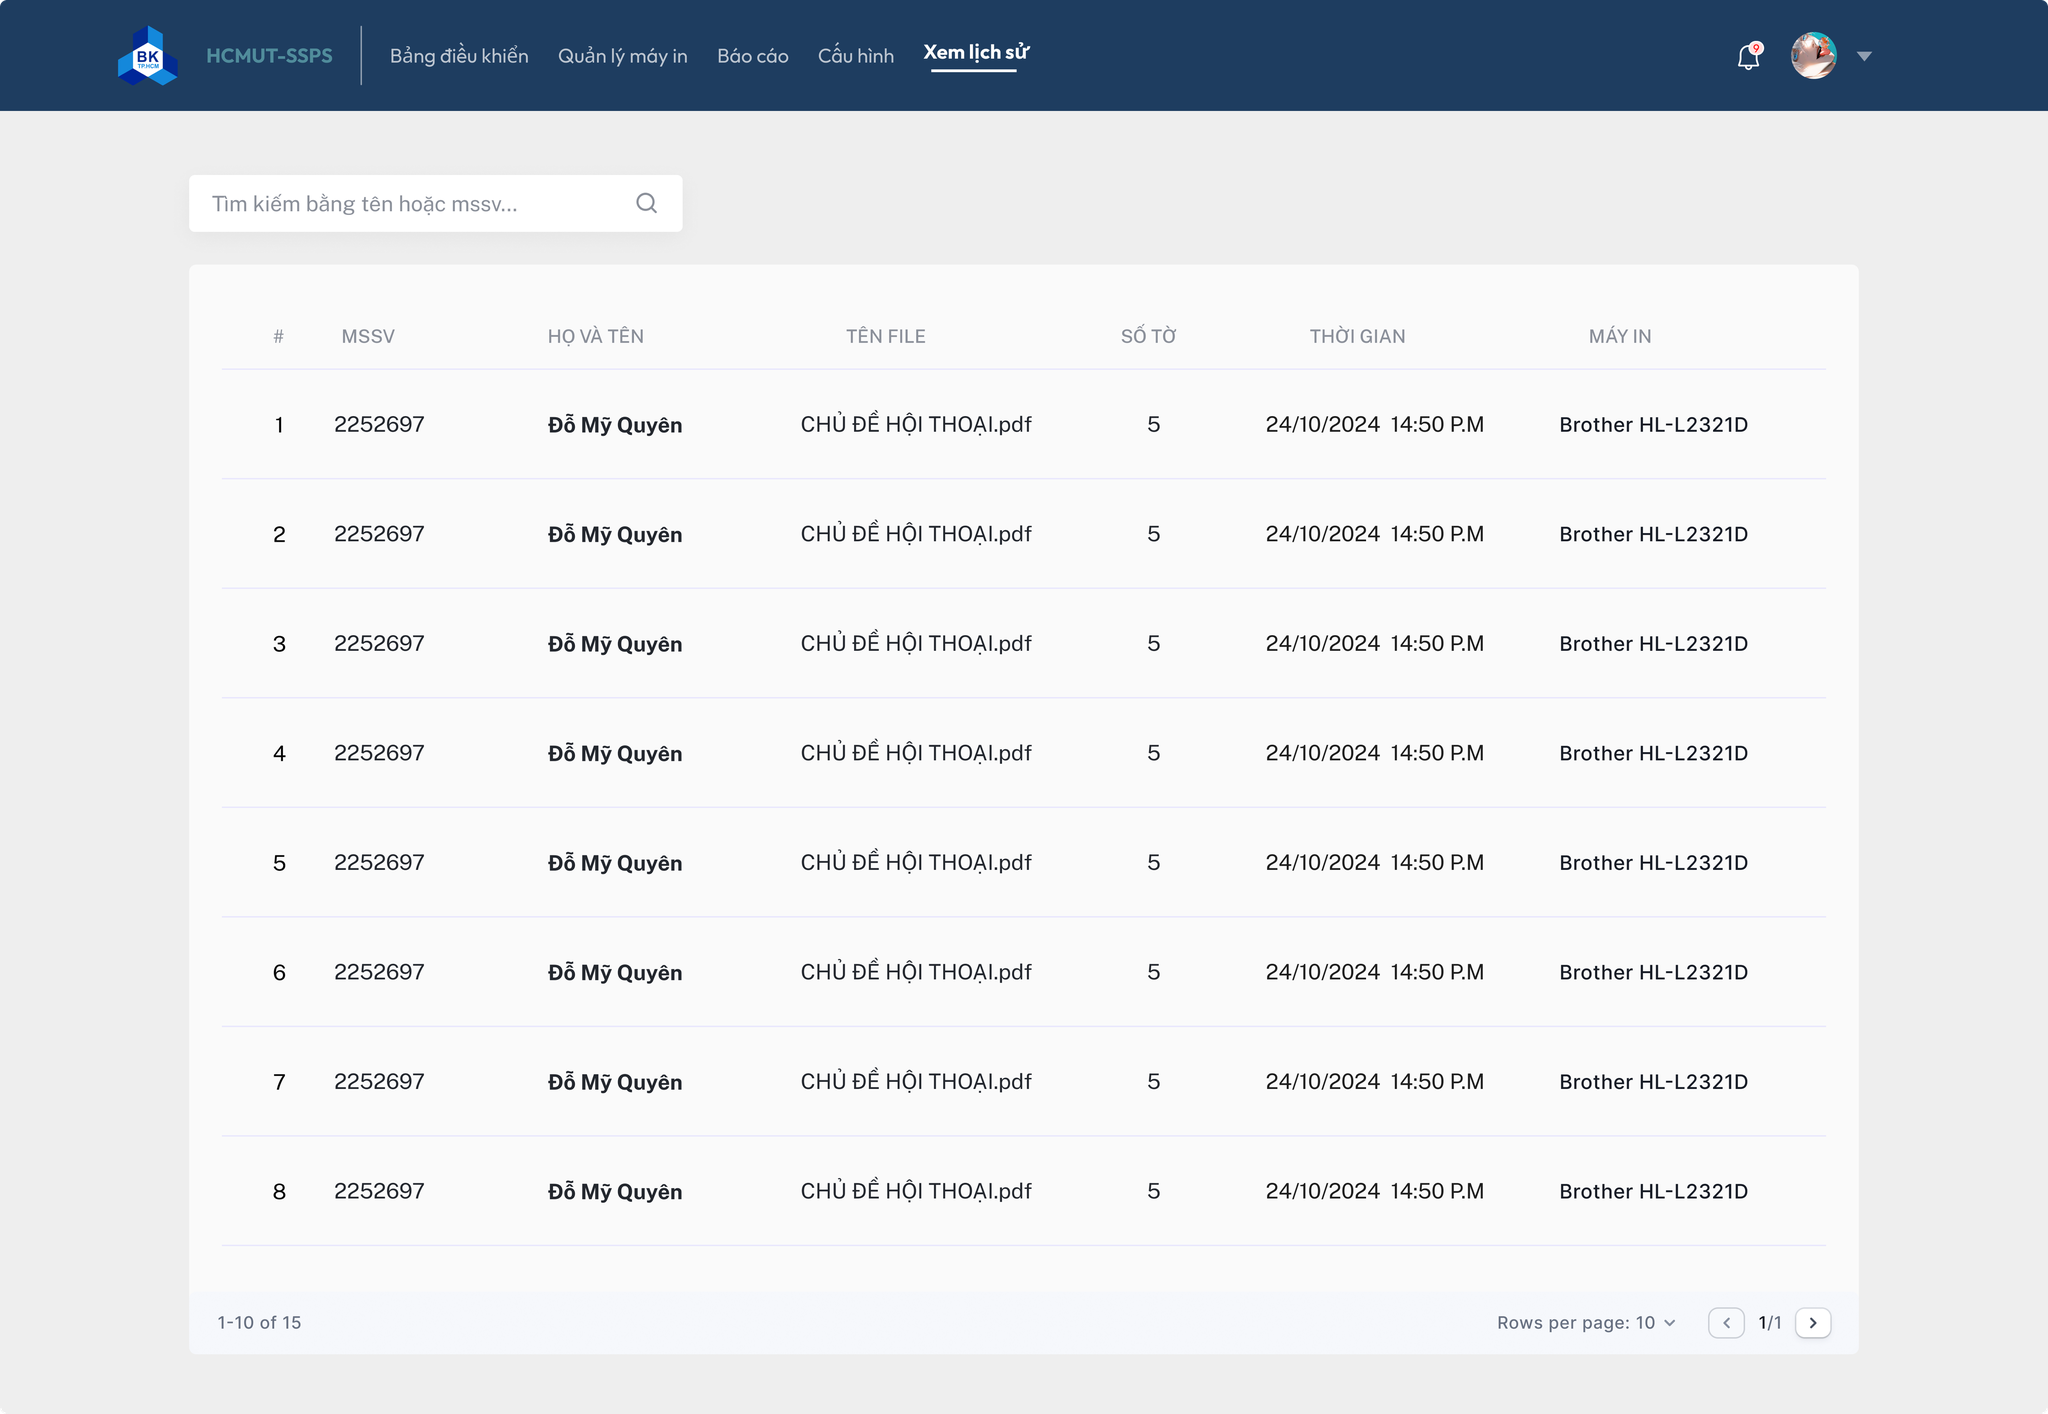
\includegraphics[width=1\linewidth]{Images/UI/View_student's_history_page.png}
     \caption{Students' Printing History Page}
 \end{figure}
\newpage
\subsection{Students}
\subsubsection{Dashboard Page}
\begin{figure}[htbp]
     \centering
     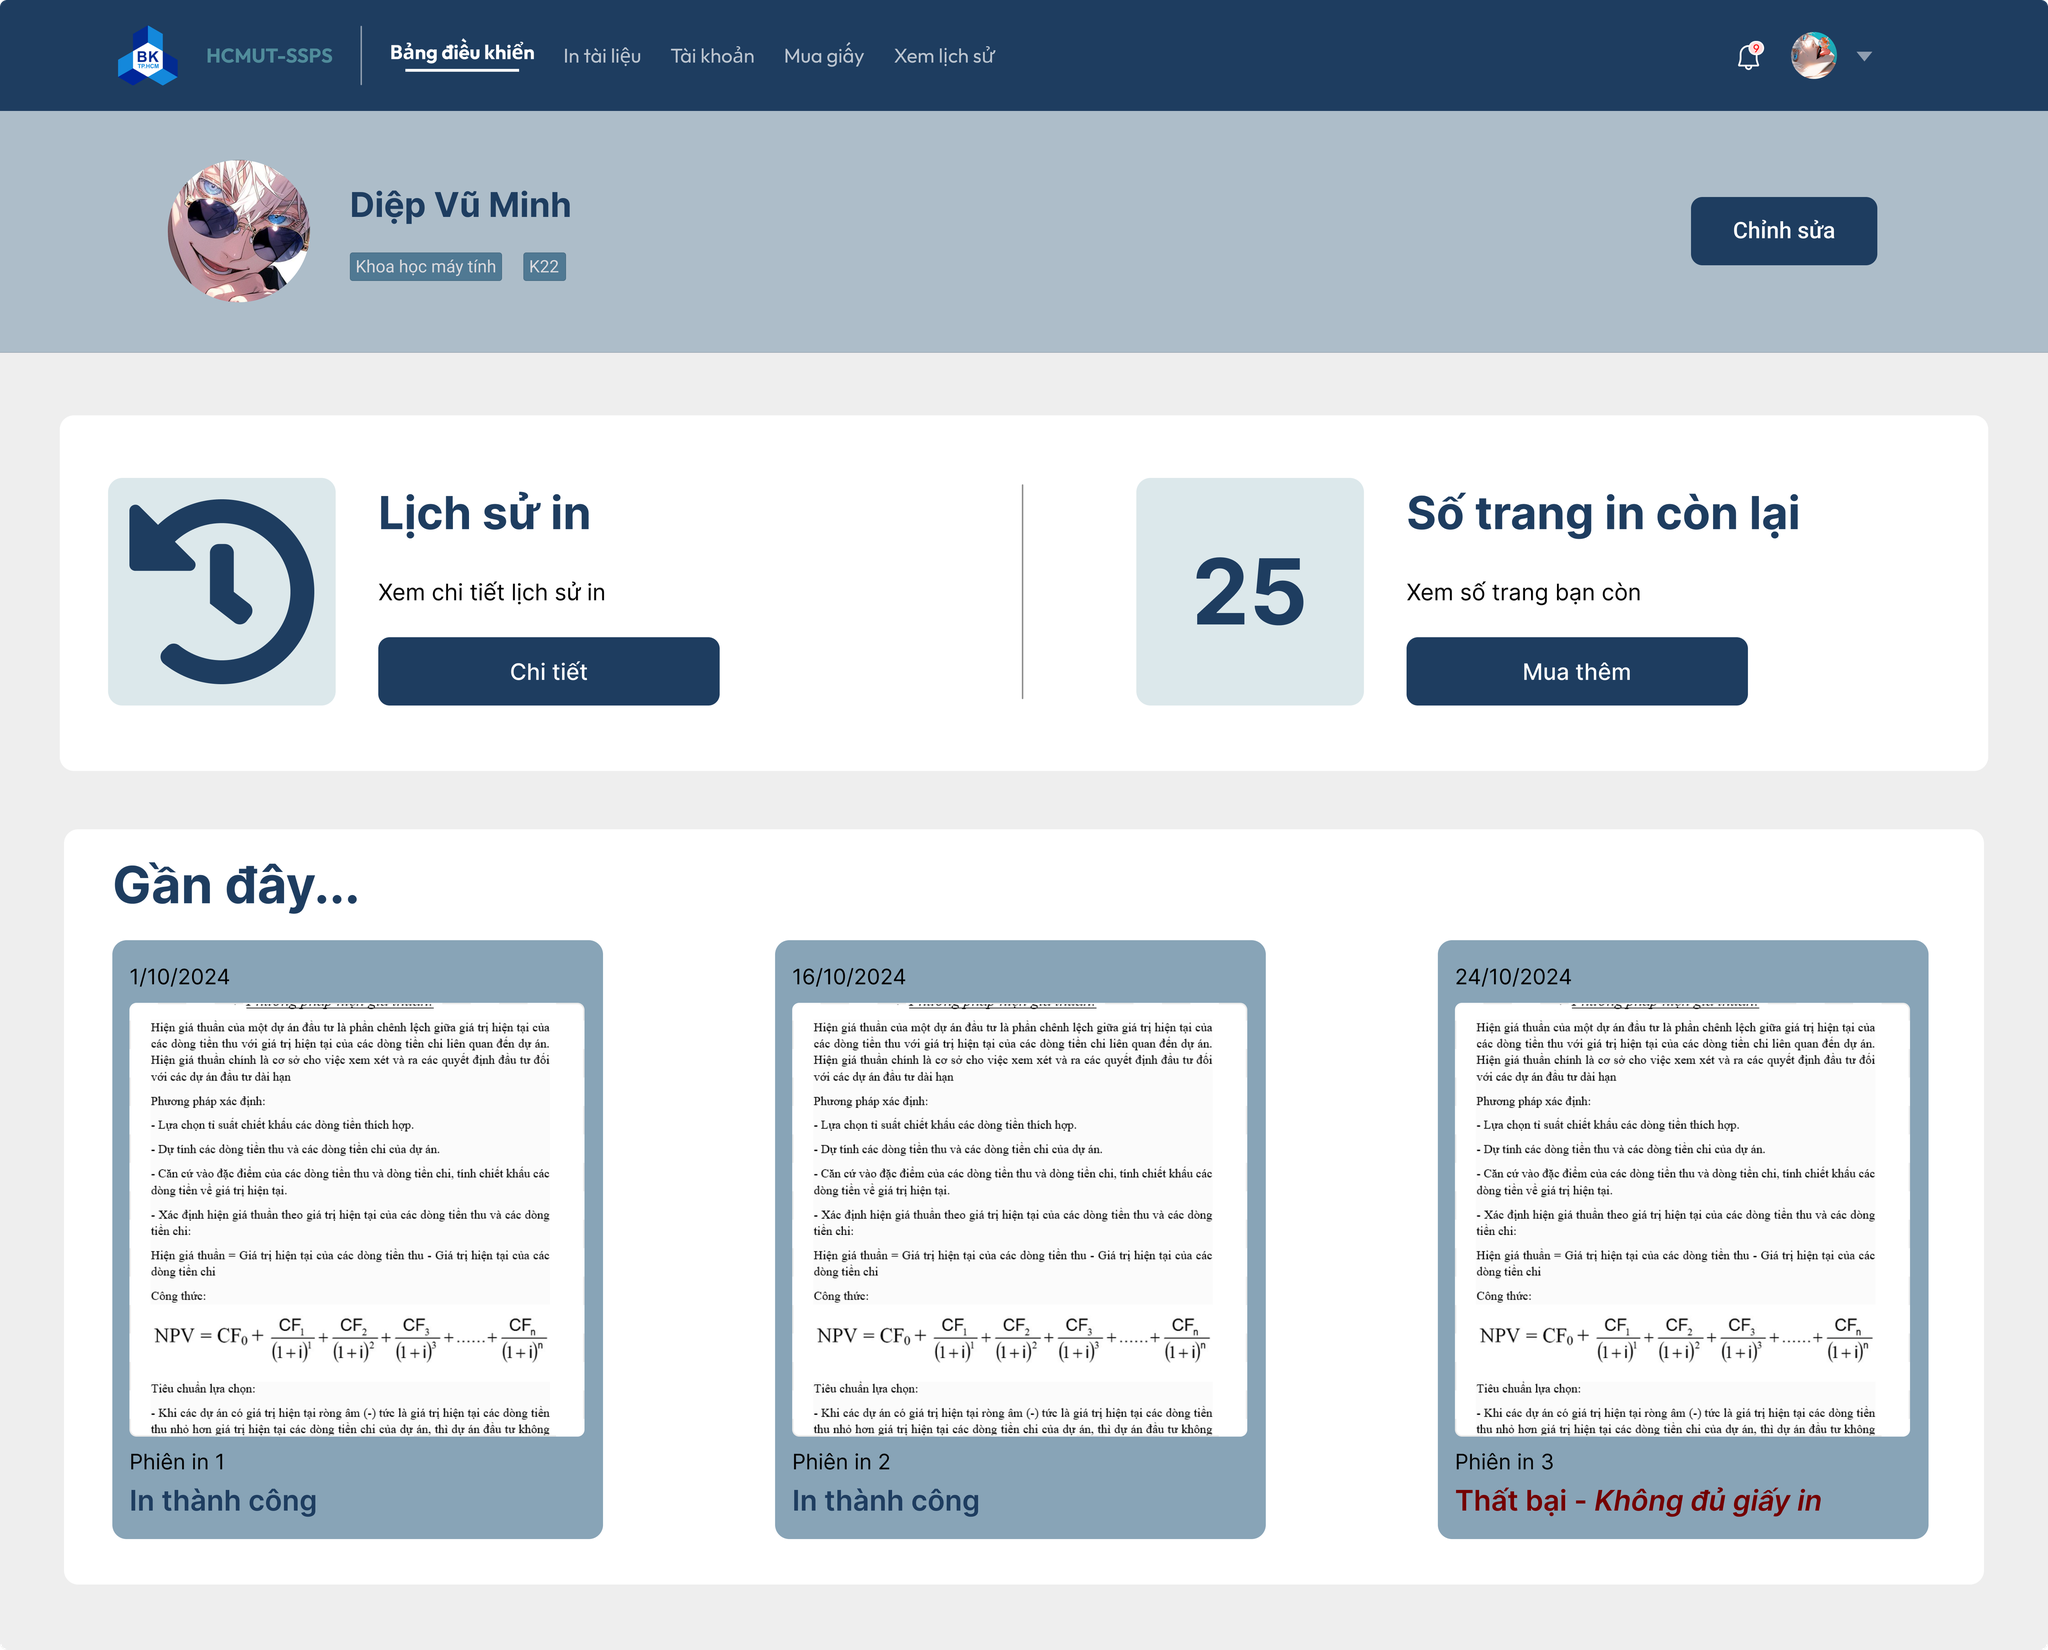
\includegraphics[width=1\linewidth]{Images/UI/Dashboard_pages.png}
     \caption{Dashboard Page}
 \end{figure}
 \newpage
\subsubsection{Print Document Page}
\begin{figure}[htbp]
     \centering
     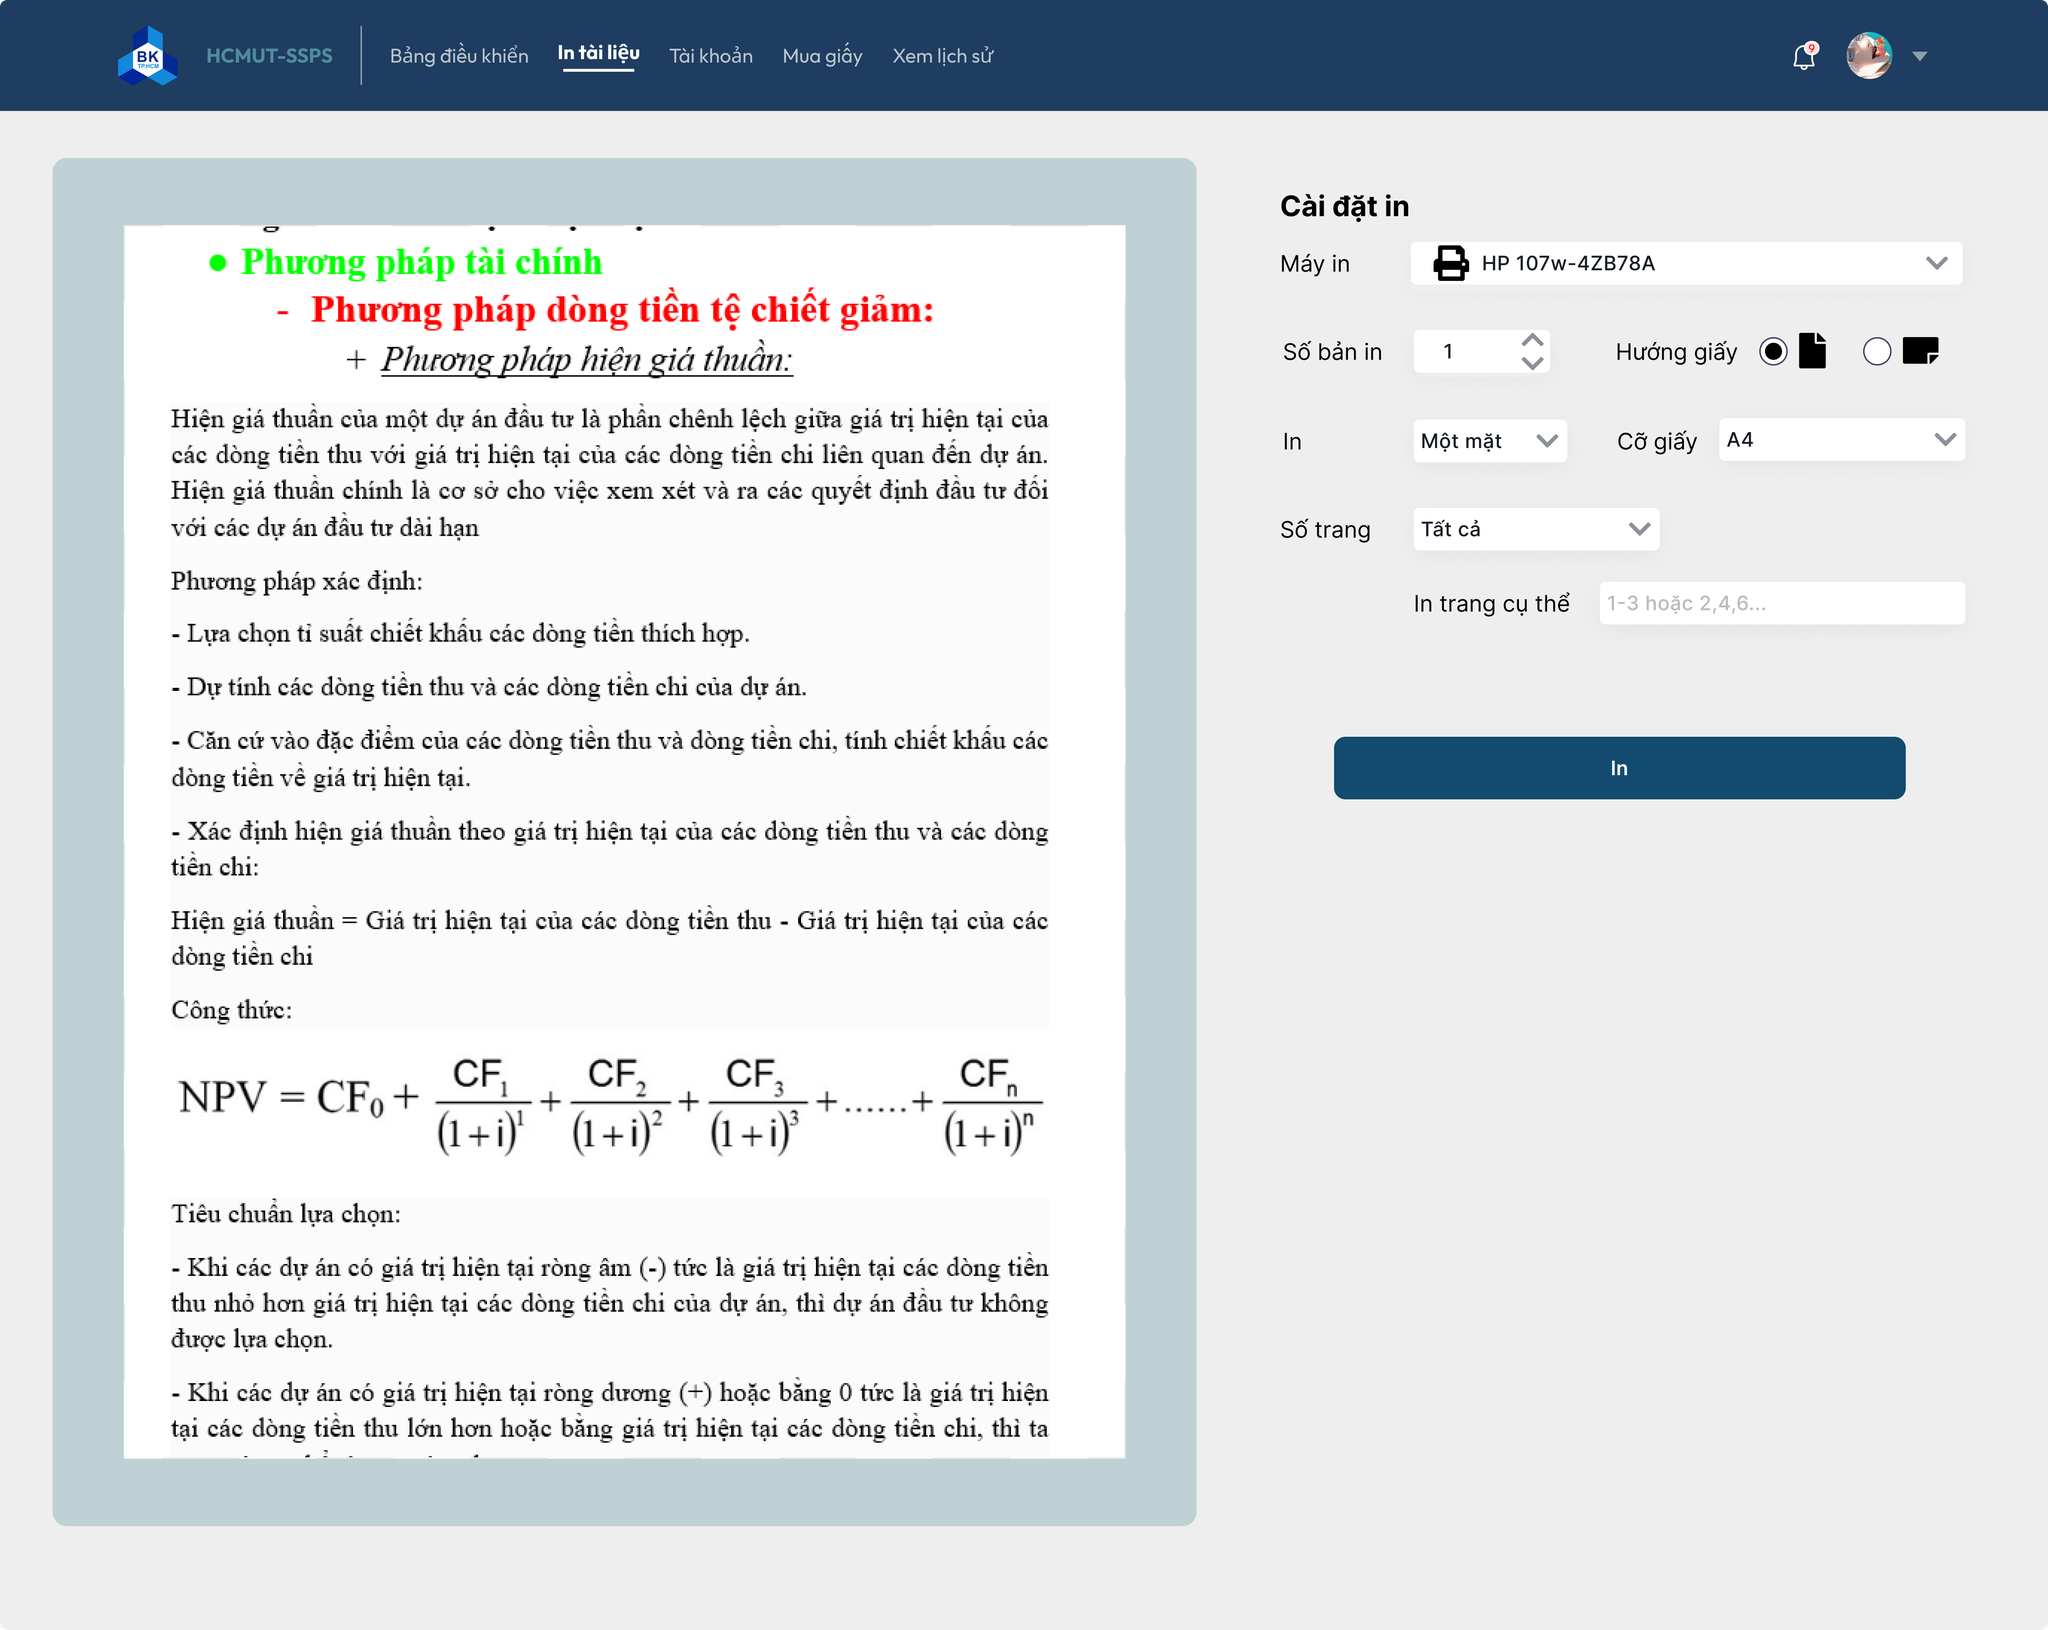
\includegraphics[width=1\linewidth]{Images/UI/Print_document_page.png}
     \caption{Print Document Page}
 \end{figure}
 \newpage
\subsubsection{Printing History Page}
\begin{figure}[htbp]
     \centering
     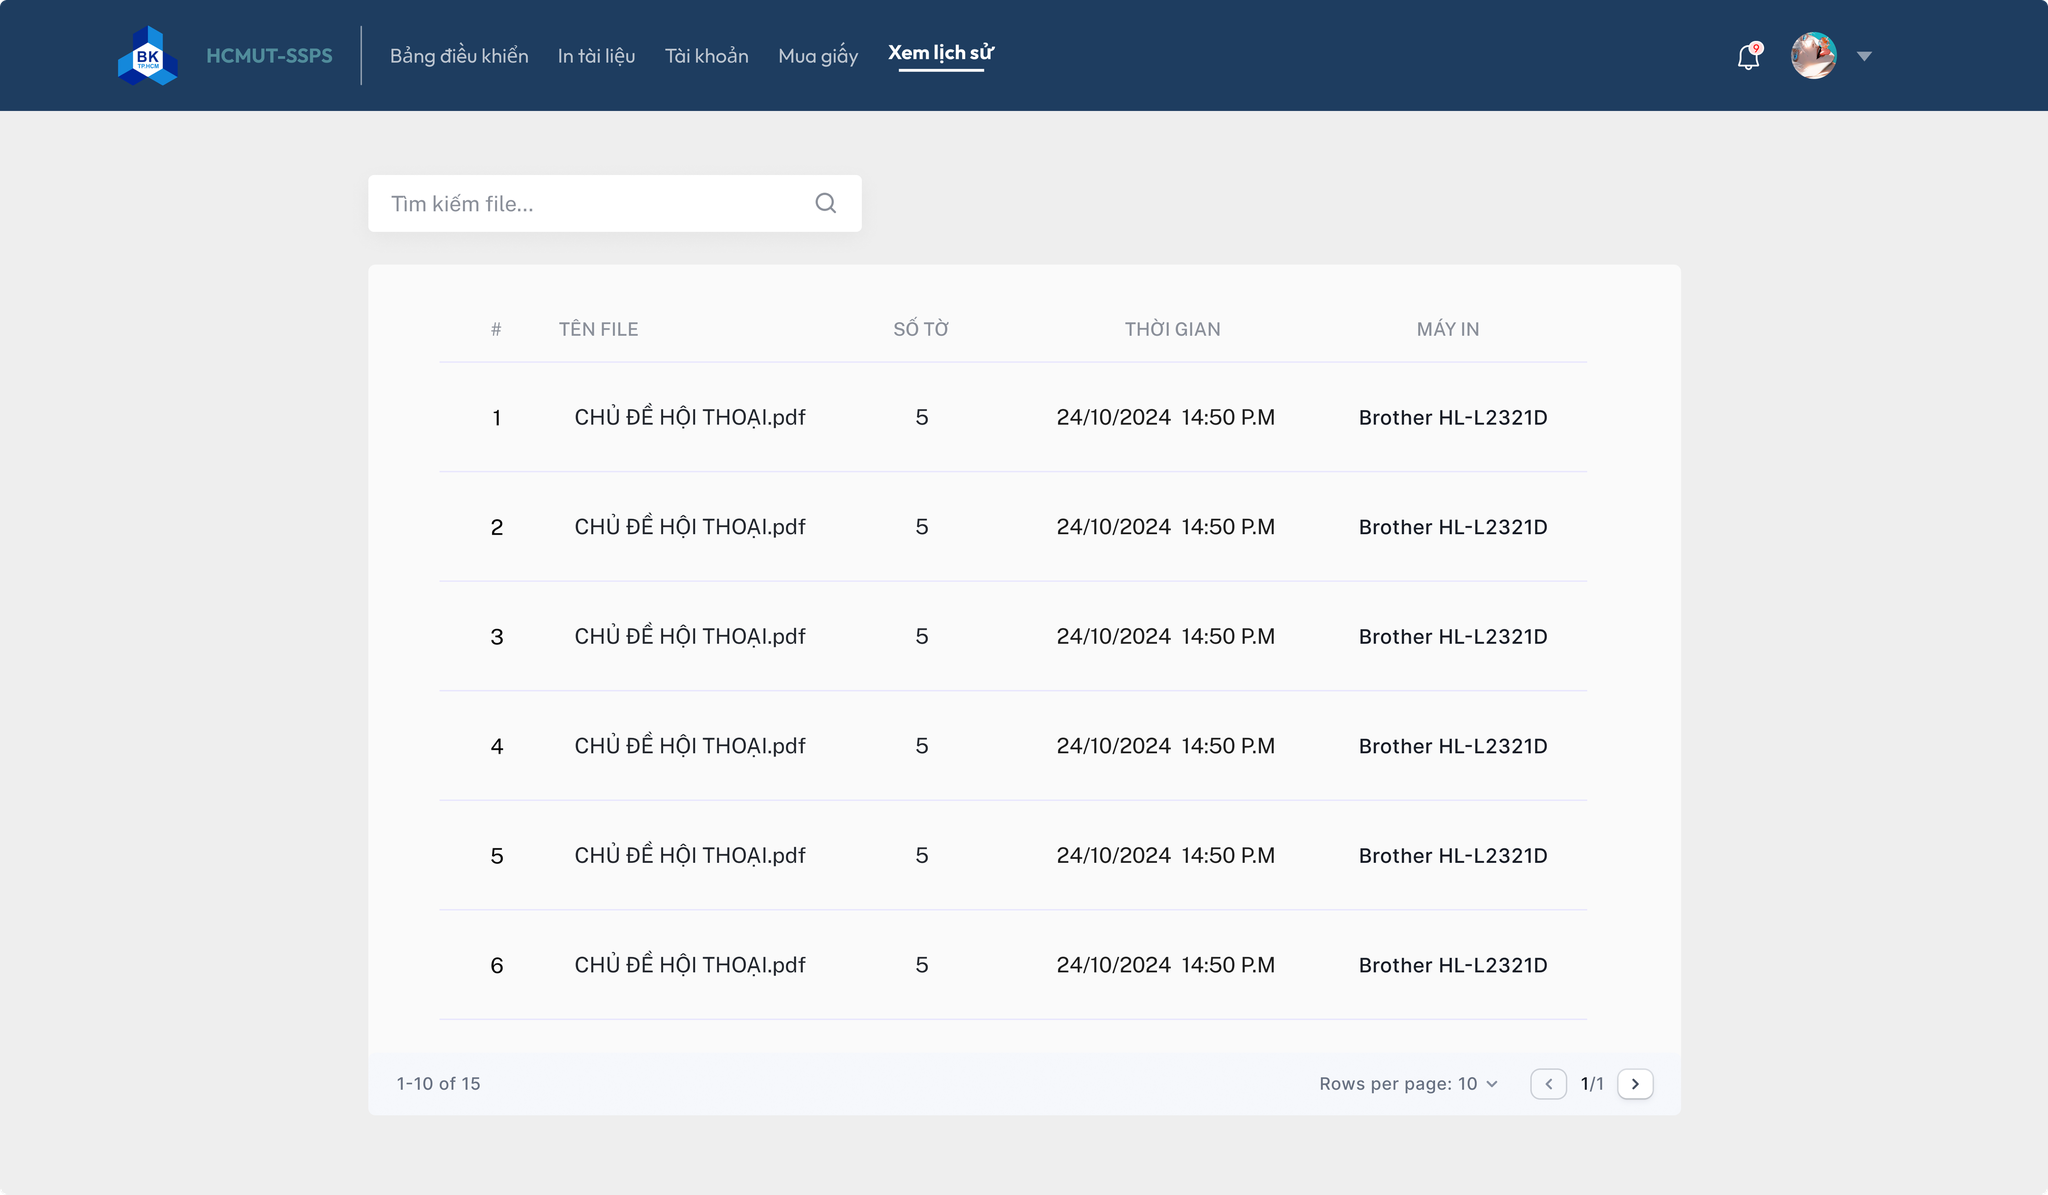
\includegraphics[width=1\linewidth]{Images/UI/Printing History Page.png}
     \caption{Printing History Page}
 \end{figure}
\subsubsection{Upload Page}
\begin{figure}[h!]
     \centering
     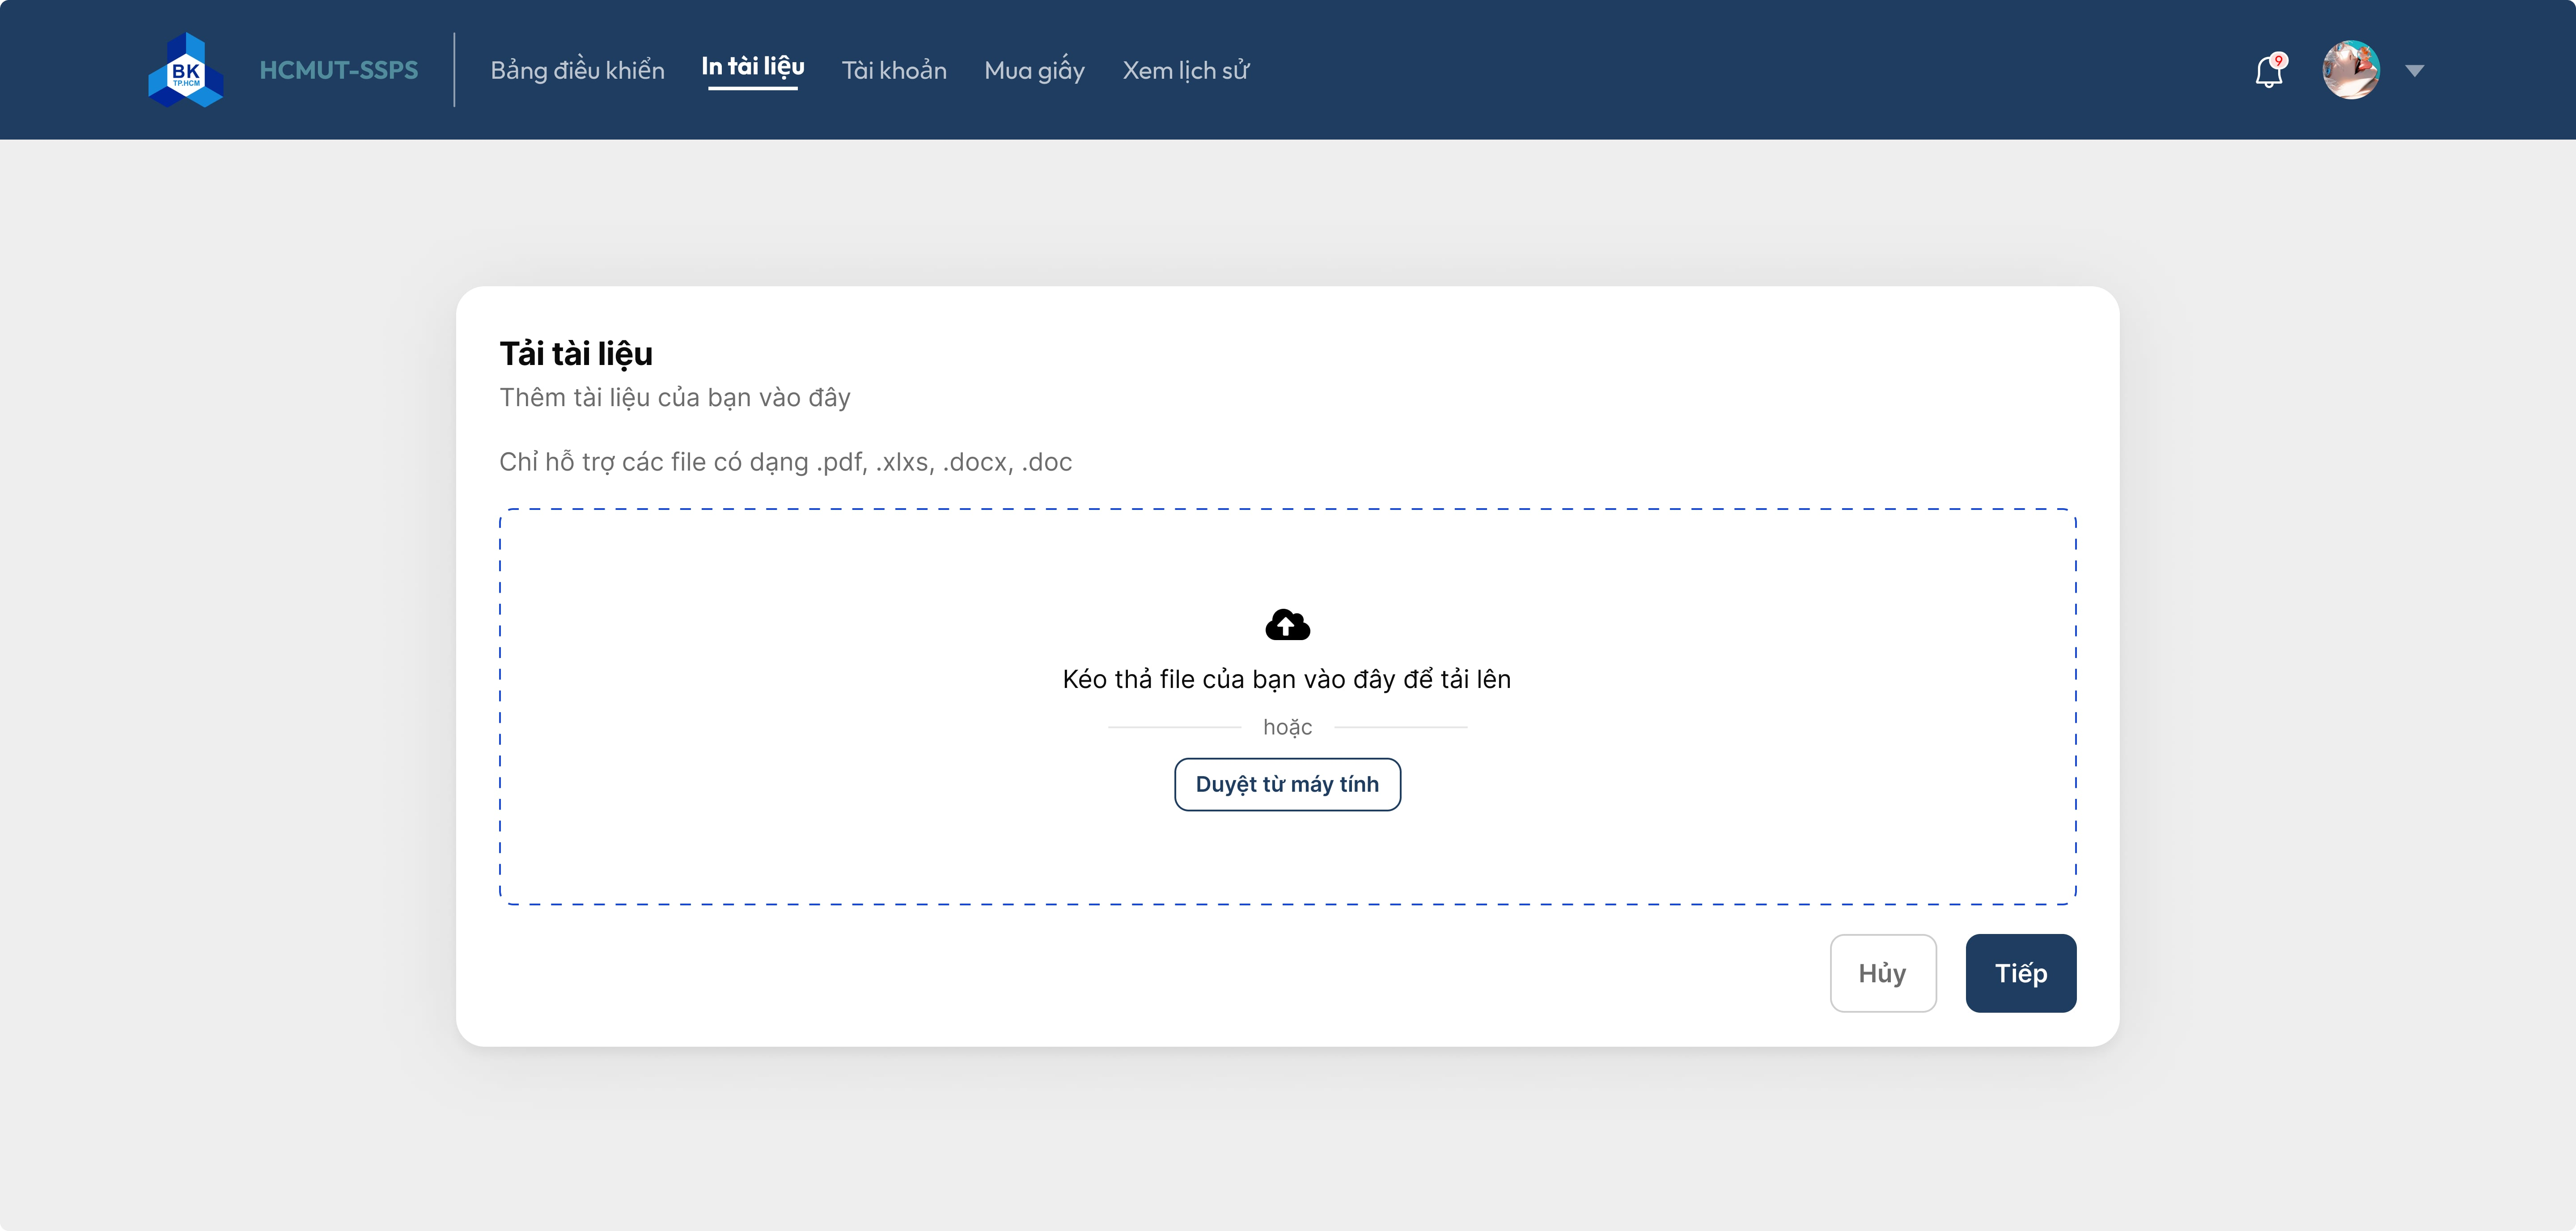
\includegraphics[width=1\linewidth]{Images/UI/Upload Page.jpg}
     \caption{Upload Page}
 \end{figure}


